\documentclass[journal]{IEEEtran}
\usepackage{amsmath,amssymb,amsthm}
\usepackage{bm}
\usepackage{graphicx}
\usepackage{booktabs}
\usepackage{float}
\usepackage[hidelinks]{hyperref}

\newtheorem{theorem}{Theorem}
\newtheorem{proposition}{Proposition}
\newcommand{\R}{\mathbb{R}}
\newcommand{\var}{\operatorname{var}}

\title{The Utah Teapot in CONV Geometry:\\ Nodes on the Surface, Rays by Transport}
\author{Anonymous}
\date{}

\begin{document}
\maketitle

\begin{abstract}
We rebuild the Utah Teapot from points that lie on its own surface. The
representation is a lattice of nodes reconstructed by Compact Ordered Nodal
Variation (CONV) with ledger-free admission. Three additions make it a
geometry and not only an image filter. Declared \emph{seams} with
cubic-exact one-sided stencils let the lattice reproduce bicubic B\'ezier
patches exactly: with four node intervals per patch, 560 on-surface nodes
reproduce the 28 original patches to $2\times10^{-15}$. A symmetric bubble
limiter replaces the standard one, which is discontinuous in the data and
can open cracks in a surface; the new limiter is continuous and keeps the
variation bound. And because a CONV cell depends on a fixed block of nodes,
the surface has a pointwise evaluator with exact derivatives. We render it
by \emph{correspondence transport}, which sends a lattice of known
parameters forward to the screen and lets each pixel correct a prediction
with a Newton step; it is 1.6 to 2.0 times faster than a per-ray tracer of
the same surface and agrees with a fine reference on 99.9\% of surface
pixels. The representation needs no patches, control points, degrees or
knots, only points on a surface, so later versions enter the same way: the
2026 Utah Teapot is rebuilt from 9 by 9 samples of each of its surfaces,
interior included. We then measure against the defects that the later
teapots were made to fix. A node lattice makes the body 233 times rounder
with the same node count, renders without a mesh, and carries the 2026
shape with normals matched to $0.11^\circ$ on average across joints. It
does not reproduce that model's curvature continuity, its trimming or its
chamfers. We report those as they are.
\end{abstract}

\begin{IEEEkeywords}
Utah Teapot, interpolating surface, variation diminishing, B\'ezier patch,
ray tracing parametric surfaces, correspondence transport.
\end{IEEEkeywords}

\section{Introduction}

The Utah Teapot was modelled by Martin Newell in 1974--75 as 28 bicubic
B\'ezier patches and scaled to its familiar proportions by Jim Blinn in
1976 \cite{newell1975,blinnnewell1976,crow1987,blinn1987}. Its control
points mostly lie off the surface: a B\'ezier patch passes through only
four of its sixteen. Every later version of the model addressed something
that the original patches leave open. Crow added a bottom. Driskill made
the body round, trimmed the handle and spout to the body and added an
interior. Fish improved the interior. Yuksel's 2026 version adds chamfers,
a lighter interior, texture layouts and curvature continuity for smooth
reflections \cite{utahpage,yuksel2026}.

This paper asks what the teapot looks like in a different kind of
representation: one whose every control value is a point of the surface.
CONV \cite{convpaper} interpolates samples on a regular lattice by a
piecewise quintic whose derivative cannot change sign more often than the
samples do. It was built for images. Used for positions, it gives a surface
through a lattice of nodes, and a node can be moved, measured, textured or
collided with as the surface point it is.

The contributions are these.
\begin{enumerate}
\item \emph{Seamed CONV lattices} (Section~\ref{sec:seams}). A seam cuts
the difference stencils along a node row or column. With cubic-exact
end stencils, a seamed lattice reproduces any piecewise bicubic surface
whose patch joints lie on seams, wherever admission leaves the proposal
alone. For the teapot it is alone everywhere.
\item \emph{A continuous bubble limiter} (Section~\ref{sec:bubble}). We
show that the standard limiter jumps, give a symmetric replacement, and
prove that it keeps the variation bound.
\item \emph{A pointwise surface evaluator and transport ray tracing}
(Sections~\ref{sec:surface} and \ref{sec:transport}), with a measured
comparison against per-ray tracing of the same surface.
\item \emph{An account against the later teapots}
(Section~\ref{sec:qualities}): what the representation improves, what it
leaves unchanged, and what it does not address.
\end{enumerate}
An engine that implements all of it accompanies the paper and runs in a
browser on one CPU thread. Its controls follow the official Utah Teapot
page: a choice of version (1975, 1976, 1987, 2026), switches for the
handle, spout, lid, body and interior, Blinn's scale, wireframe, texture
coordinates per part or per patch, and reflection lines; it adds gloss
and a rigid-body drop.

\subsection{For readers of the spline literature}

CONV on a lattice is an \emph{interpolating} surface formulation, and the
questions usually put to one have short answers here.
\begin{itemize}
\item \emph{Interpolation.} The surface passes through every node. There
are no off-surface controls and no handles.
\item \emph{Locality and cost.} A cell depends on the six samples around
it in each direction (eight next to a seam). Every step is closed form,
with constant work per cell and no global solve.
\item \emph{Precision.} Linear data are reproduced exactly, so straight
pieces need no special constraint. With seams, cubics are reproduced
exactly (Proposition~\ref{prop:cubic}).
\item \emph{Continuity.} $C^2$ across node lines wherever the limiter is
inactive; $C^0$ across a seam, which is how a crease is modelled.
Curvature is not controlled at a seam, and Section~\ref{sec:qualities}
measures what that costs.
\item \emph{Shape.} The derivative along a line changes sign no more often
than the samples do. Overshoot next to a crease or a step is excluded by
construction, not by tuning.
\item \emph{Dependence on the data.} Continuous and piecewise affine in the
nodes (Theorem~\ref{thm:symmetric}).
\item \emph{What it lacks.} Samples are taken as uniformly spaced in the
parameter. Coordinates are limited separately, so where the limiter acts
the surface is not rotation invariant. It is not a subdivision or a
convex-hull scheme.
\end{itemize}

\section{CONV Lines}

We restate what is needed from \cite{convpaper}. For samples $y_i$ on a
line, with secants $\delta_i=y_{i+1}-y_i$, each node receives a scaled jet
$(m_i,q_i)$ from a difference stencil. The cell $[i,i+1]$ gets five raw
currents, the differences of six quintic B\'ezier controls:
\begin{align}
 a_{i0}&=\tfrac{m_i}{5}, & a_{i1}&=\tfrac{m_i}{5}+\tfrac{q_i}{20},\nonumber\\
 a_{i4}&=\tfrac{m_{i+1}}{5}, & a_{i3}&=\tfrac{m_{i+1}}{5}-\tfrac{q_{i+1}}{20},
 \label{eq:raw}
\end{align}
and $a_{i2}=\delta_i-a_{i0}-a_{i1}-a_{i3}-a_{i4}$. Ledger-free admission
clips $a_i$ into a box built from the two neighbouring secants and
terminal currents, and restores the cell mass $\delta_i$ by one capped
common shift. The admitted currents $c_i$ satisfy
$\var(c^\flat)\le\var(\delta)$ for \emph{any} proposal whose cells sum to
their secants; the proof in \cite{convpaper} uses nothing else. The cell
is then
\begin{equation}
 y(i+t)=y_i+\sum_{j=0}^{4}c_{ij}\,\tau_j(t)+\omega_i\,\psi(t),
 \label{eq:cell}
\end{equation}
with $\tau_j=\sum_{r>j}B_r^5$ and the odd bubble
$\psi(t)=[t(1-t)]^3(2t-1)$. In the interior of a line the jets are the
fourth-order centred stencils, and a cell depends on the six samples
$y_{i-2},\ldots,y_{i+3}$ only.

\section{Seams and Cubic Precision}
\label{sec:seams}

A first attempt to put the teapot on a plain CONV lattice fails near its
creases and patch joints. With four node intervals per patch the worst
deviation from the B\'ezier surface is $5.9\times10^{-2}$ on a body 4.0
wide, against $1.05\times10^{-1}$ for the same nodes joined bilinearly;
next to the crease of a flat bottom cap, CONV is \emph{worse} than linear.
The variation bound holds, and there is no overshoot. The loss is in the
jets: a centred stencil that straddles a crease measures a slope that
belongs to neither side.

\subsection{Seams}

A \emph{seam} is a node row or column across which no difference stencil
may reach. Values remain continuous across it. The two ends of an open
line are seams; a closed ring without seams is periodic. A node on a seam
has two jets, one from each side. For a segment of at least four nodes
between seams we use the stencils that are exact for cubics and still fit
the six-sample window:
\begin{align}
 m_0&=\tfrac16(-11y_0+18y_1-9y_2+2y_3),\nonumber\\
 q_0&=2y_0-5y_1+4y_2-y_3,\nonumber\\
 m_1&=\tfrac16(-2y_0-3y_1+6y_2-y_3),\label{eq:closure}\\
 q_1&=y_0-2y_1+y_2,\nonumber
\end{align}
with their mirror images at the other end and the centred stencils from
the third node on. Admission is unchanged, except that the terminal
current a cell sees in its neighbour across a seam, $a_{i-1,4}$ or
$a_{i+1,0}$, is now the neighbour's own one-sided value. This is the case
for which the knot-exclusivity terms of the box were written; without
seams they collapse to the sign of a shared slope. A cell next to a seam
depends on $y_{i-3},\ldots,y_{i+4}$.

\begin{proposition}[Cubic precision]
\label{prop:cubic}
Let a segment between two seams have at least four nodes, and let its
samples be those of a cubic polynomial at equally spaced parameters. If
admission leaves every raw current of the segment unchanged, the CONV
line equals that cubic on the segment, with zero bubble.
\end{proposition}

\begin{proof}
The stencils \eqref{eq:closure} and the centred stencils return the first
and second derivatives of a cubic exactly. The raw quintic of each cell
is then the quintic Hermite interpolant of exact two-jets of a cubic at
both ends, which is that cubic. With $c_i=a_i$ the second term of the
bubble fit vanishes, and its first term is a fifth difference, which
vanishes on a cubic.
\end{proof}

\begin{theorem}[Exact B\'ezier reproduction]
\label{thm:exact}
Let a surface be a grid of bicubic B\'ezier patches, sampled at $n\ge3$
equal parameter intervals per patch in each direction, with seams on
every patch boundary. If admission is inactive in both factors, the CONV
surface of Section~\ref{sec:surface} equals the B\'ezier surface.
\end{theorem}

\begin{proof}
Along a node row inside one patch the samples are those of a cubic, so by
Proposition~\ref{prop:cubic} every row line equals the surface along that
row at every $u$. The second factor then interpolates, at fixed $u$,
values that are samples of the cubic $v\mapsto S(u,v)$ within the patch.
\end{proof}

The hypothesis is checkable, and for the teapot it holds.
Table~\ref{tab:exact} gives the measured deviation at eight samples per
node interval over all four parts. From four intervals per patch on, the
teapot's own geometry passes admission untouched and the two surfaces
agree to rounding. At three intervals a few cells are clipped. At two
there are too few nodes for a cubic stencil.

\begin{table}[H]
\caption{Deviation from the B\'ezier teapot (body 4.0 wide)}
\label{tab:exact}
\centering
\scriptsize
\begin{tabular}{rr|cc|cc}
\hline
 & & \multicolumn{2}{c|}{Seamed, cubic ends} & \multicolumn{2}{c}{Seamless}\\
$n$ & Nodes & max & rms & max & rms\\
\hline
2 & 152 & $2.3\times10^{-1}$ & $5.4\times10^{-2}$ & $2.1\times10^{-1}$ & $4.8\times10^{-2}$\\
3 & 324 & $2.9\times10^{-5}$ & $1.3\times10^{-6}$ & $8.8\times10^{-2}$ & $1.7\times10^{-2}$\\
4 & 560 & $2.3\times10^{-15}$ & $4.1\times10^{-16}$ & $5.9\times10^{-2}$ & $9.5\times10^{-3}$\\
6 & 1224 & $3.4\times10^{-15}$ & $6.2\times10^{-16}$ & $3.5\times10^{-2}$ & $4.7\times10^{-3}$\\
8 & 2144 & $2.4\times10^{-15}$ & $4.1\times10^{-16}$ & $2.5\times10^{-2}$ & $2.9\times10^{-3}$\\
\hline
\end{tabular}
\end{table}

The node count is not smaller than the control-point count; 28 patches
have 448 control points and the exact lattice has 560 nodes, 64 of them on
a flat bottom cap that is not one of the 28 patches. What changes is
where they are. All 560 are points of the teapot.

\section{A Continuous Bubble}
\label{sec:bubble}

The bubble amplitude $\omega_i$ is fitted and then limited so that the
degree-six Bernstein coefficients of the cell's derivative keep their
signs. Writing $d_2,d_3,d_4$ for the three coefficients the bubble
touches, the enriched ones are $d_2-\omega/5$, $d_3+2\omega/5$ and
$d_4-\omega/5$. The standard limiter \cite{convpaper} lets each keep its
sign \emph{one-sidedly}: for $d_2>0$ it requires only $\omega\le5d_2$.

\begin{proposition}[The standard limiter is discontinuous]
Fix a fitted amplitude $\widehat\omega>0$ and let $d_2$ pass through zero
with $d_3,d_4$ fixed and nonzero. For $d_2\downarrow0$ the admitted
amplitude tends to $0$. For $d_2\uparrow0$ the constraint from $d_2$ is a
lower bound that tends to $0$, and the admitted amplitude tends to
$\min\{\widehat\omega,U\}$, where $U>0$ is the upper bound from the other
two coefficients whenever one exists.
\end{proposition}

On a line this is a jump in the data-to-value map. On a surface it is a
crack: the second factor's inputs vary continuously with $u$, and where
one of its coefficients changes sign the surface position jumps. The
defect was observed in an earlier cloth experiment; here is its cause and
a cure.

\begin{theorem}[Symmetric limiter]
\label{thm:symmetric}
Let
\begin{align}
 M_i&=\min\{5|d_{i2}|,\ \tfrac52|d_{i3}|,\ 5|d_{i4}|\},\nonumber\\
 \omega_i&=\max\{-M_i,\min\{M_i,\widehat\omega_i\}\}.
 \label{eq:symmetric}
\end{align}
Then $\omega_i$ is a continuous piecewise-affine function of the cell's
samples, no enriched coefficient changes sign, and the variation bound of
\cite{convpaper} holds unchanged. Wherever
$|\widehat\omega_i|\le M_i$ the amplitude equals the fitted one, so the
leading-error reduction $1681/1950$ is retained.
\end{theorem}

\begin{proof}
$|\omega_i|\le M_i$ gives $|\omega_i/5|\le|d_{i2}|$,
$|2\omega_i/5|\le|d_{i3}|$ and $|\omega_i/5|\le|d_{i4}|$, so each
enriched coefficient is zero or has the sign of the one it replaces. That
is the only property of the amplitude used in the variation proof.
$\widehat\omega_i$ is linear in the samples and the admitted currents,
which are continuous and piecewise affine; $M_i$ is a minimum of absolute
values of linear forms of them; and a clamp is continuous in its three
arguments.
\end{proof}

The symmetric bound is the tighter of the two, since it limits both signs
of the amplitude. On resolved smooth data the fit is of fifth order in the
spacing and the coefficients of first order, so neither limiter acts and
the two agree. Table~\ref{tab:jump} measures the difference where it
matters: the largest change of position between surface samples one step
apart along $u$, on the teapot body with its nodes displaced by noise of
standard deviation 0.08. A continuous surface gives a change proportional
to the step. The standard limiter leaves a jump of $1.3\times10^{-4}$ at a
step of $10^{-6}$, about a hundred times the continuous value.

\begin{table}[H]
\caption{Largest position change over one parameter step}
\label{tab:jump}
\centering
\scriptsize
\begin{tabular}{l|cc}
\hline
Bubble & step $10^{-4}$ & step $10^{-6}$\\
\hline
off        & $1.8\times10^{-3}$ & $1.4\times10^{-6}$\\
standard   & $2.0\times10^{-3}$ & $1.3\times10^{-4}$\\
symmetric  & $1.9\times10^{-3}$ & $1.4\times10^{-6}$\\
\hline
\end{tabular}
\end{table}

With the symmetric limiter the whole factor, bubble included, is
continuous in the data, and the surface of the next section is watertight
within each part.

\section{The Surface}
\label{sec:surface}

A part is a lattice of nodes $P_{kl}\in\R^3$, closed around ($u$) and open
along ($v$). The surface is the fixed-order composition of two CONV
factors, evaluated at a point. For $(u,v)$ in cell $(i,j)$ with local
parameters $(s,t)$:
\begin{enumerate}
\item for each node row $l=j-3,\ldots,j+4$ that exists, evaluate the
row's CONV cell $i$ at $s$, giving $R_l(s)$;
\item admit one CONV cell along $v$ from the window $R_{j-3},\ldots,R_{j+4}$
and evaluate it at $t$.
\end{enumerate}
Each coordinate is treated separately in the object's own frame. The
admitted currents of step~1 do not depend on $s$ and are compiled once
per lattice; step~2 is admitted at every query, because its inputs depend
on $u$. A point costs 24 polynomial evaluations and three admissions.
This is exactly the ordered composition of \cite{convpaper}, not an
approximation of it; the ledger form could not be evaluated this way,
since its sign ledger needs the whole line.

\emph{Derivatives.} Admission is piecewise affine, so forward-mode
differentiation through its minima and maxima is exact wherever a
derivative exists. We evaluate both steps on dual numbers that carry
$\partial/\partial s$ and $\partial/\partial t$ and obtain $S_u$ and $S_v$
with the point. The normal is their cross product.

\emph{Regularity.} Within a part the surface is continuous
(Theorem~\ref{thm:symmetric}). Where admission and the limiter are
inactive it is $C^2$ across node lines away from seams, because adjacent
cells share two-jets and $\psi$ has triple zeros. Across a seam it is
$C^0$ by design.

\emph{Invariance.} Each factor commutes with translation and with scaling
of a coordinate, so an axis-aligned affine map of the nodes maps the
surface exactly; Blinn's vertical scaling of Newell's teapot is such a
map. Where admission is inactive the operator is linear and commutes with
every affine map. Where it is active, a rotation of the nodes does not in
general rotate the surface, since coordinates are admitted separately.

\section{The Teapot}

The source is the original data from the Utah Model Repository
\cite{utahdata}: 28 patches, without a bottom. They assemble into four
parts, each a grid of patches closed around: the body (rim, upper and
lower body: four patches around, three along), the lid (knob and lid:
four by two), the handle and the spout (two half tubes around, two
along). We add an optional flat cap under the body, as Blinn suggested
\cite{blinn1987}; it meets the body at a $90^\circ$ crease, which a seam
keeps exactly, and the lowest point of the CONV body is the plane itself.

Three lattice styles are provided for this data.
\begin{itemize}
\item \emph{Exact}: seams on every patch boundary, nodes at equal
B\'ezier parameters. This is the 1976 teapot to rounding
(Table~\ref{tab:exact}).
\item \emph{Round}: as exact along $v$, but every ring of the body and
lid lies on a true circle and is closed without seams.
\item \emph{Seamless}: no seams, the closure of \cite{convpaper}. Smooth
across the patch joints, at the deviation of Table~\ref{tab:exact}.
\end{itemize}

\subsection{Other versions, from samples alone}

Nothing in Section~\ref{sec:surface} asks where the nodes came from. The
official page generates meshes of every version, and a mesh vertex of a
patch is a point of its surface. We took, for the 2026 version, the
$9\times9$ vertices of each of its 66 untrimmed surfaces at eight intervals
per patch, and for the 1987 version the four patches of Crow's round
bottom. Symmetry leaves 19 distinct patches of the 66. Each becomes one
open lattice with cubic ends. No control point, degree, knot vector or
continuity construction of the source model is used or known to us; the
samples are not even uniform in the source parameter.

The versions offered are then: \emph{1975}, Newell's proportions, which is
the 1976 lattice with its heights scaled by $4/3$, an exact operation
(Section~\ref{sec:surface}); \emph{1976}; \emph{1987}, the 1976 lattice
raised by 0.15 with the sampled bottom; and \emph{2026}, 5346 nodes on 46
exterior and 20 interior surfaces. Adjacent lattices share their edge
samples, and a CONV line along an edge depends on that edge's samples
alone, so the lattices meet without gaps: the largest measured gap over
52 joints is $9\times10^{-8}$, the rounding of the single-precision
samples. Fig.~\ref{fig:versions} shows them.

What is left out is stated plainly. The 2026 model trims the body, handle
and spout against each other and adds chamfers at the joins; those
surfaces come out of the generator as irregular meshes, not grids, and
are not included, so the handle and spout still pass through the wall.
The 1992 and 2006 versions, whose difference is in trimmed surfaces and
interiors, are not included.

\begin{figure*}[t]
\centering
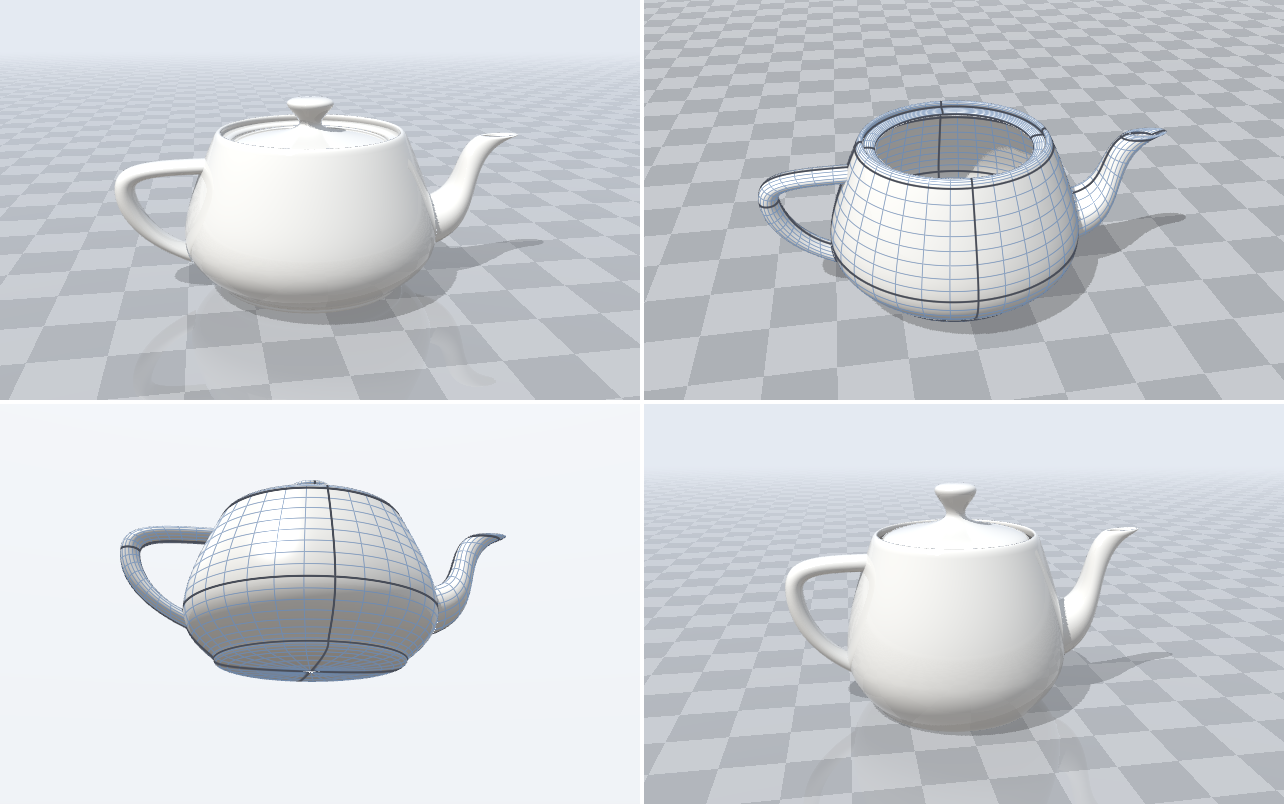
\includegraphics[width=0.86\textwidth]{figures/fig_versions.png}
\caption{Versions as node lattices. Top: the 2026 version from surface
samples, glazed; the same with the lid removed, showing its interior and
the node lines of each $9\times9$ lattice. Bottom: the 1987 version from
below, with Crow's round bottom; the 1975 version in Newell's
proportions.}
\label{fig:versions}
\end{figure*}

\section{Against the Later Teapots}
\label{sec:qualities}

Each later version fixed a named defect. We take them in turn and say
what a node lattice does about each. Table~\ref{tab:qualities} is the
summary; the measurements follow.

\begin{table}[H]
\caption{Defects addressed by later versions, and by a CONV lattice}
\label{tab:qualities}
\centering
\scriptsize
\begin{tabular}{p{2.55cm}|p{1.55cm}|p{3.4cm}}
\hline
Defect of the 1976 patches & Fixed in & CONV lattice\\
\hline
Body not round & 1992 & Improved: 233 times rounder at the same node count\\
Kinked knob tip & mesh options & Improved: the kink is removed\\
No bottom & 1987 & Flat cap with an exact crease; Crow's round bottom from samples\\
Curvature jumps at patch joints & 2026 & Shape carried from samples; continuity itself not reproduced, see below\\
Handle and spout pierce the body & 1992, 2026 & Not addressed\\
No interior & 1992--2026 & The 2026 interior, from samples\\
Gap around the lid & 1992 & Not addressed\\
Mesh cracks, duplicate vertices, pole triangles & mesh options & Not applicable: no mesh is made\\
Texture layout & 2026 & One chart per part; patch coordinates also offered\\
\hline
\end{tabular}
\end{table}

\subsection{Roundness}

A cubic B\'ezier arc is not a circle, and the teapot's quarter arcs use a
rounded handle length. At its widest ring the original body is out of
round by $(r_{\max}-r_{\min})/\bar r=4.1\times10^{-3}$. A node lattice
needs no new patch type to do better: put the ring's nodes on the circle.
A seamless periodic CONV ring through them is not a circle either, but
its error falls quickly with the node count (Table~\ref{tab:round}).
With the 16 nodes per turn of the exact lattice it is 233 times rounder
than the original, and the body and lid stay within $4.3\times10^{-5}$ of
the exactly revolved profile. Because the profile factor is linear in the
radius, the profile itself remains exact in this style.

\begin{table}[H]
\caption{Out-of-roundness of the body at its widest ring}
\label{tab:round}
\centering
\scriptsize
\begin{tabular}{l|c}
\hline
Surface & $(r_{\max}-r_{\min})/\bar r$\\
\hline
B\'ezier original, and CONV exact & $4.1\times10^{-3}$\\
CONV round, 12 nodes per turn & $9.6\times10^{-5}$\\
CONV round, 16 nodes per turn & $1.7\times10^{-5}$\\
CONV round, 24 nodes per turn & $1.6\times10^{-6}$\\
CONV round, 32 nodes per turn & $2.8\times10^{-7}$\\
\hline
\end{tabular}
\end{table}

The same change repairs the knob tip. The original lid ends in a ring of
radius 0.01 whose four quarter patches meet at a kink: the tangent
around the ring turns by $18.9^\circ$ a seventh of a node interval below
the tip and by more nearer to it. Meshing options exist on the official
page for such tips. On the round lattice the ring is a circle and the
turn is zero.

\subsection{Curvature continuity}

Curvature continuity is the contribution of the 2026 model
\cite{yuksel2026}: where two patches of the original meet with matching
tangents but different curvature, a reflection bends. Fig.~\ref{fig:reflect}
repeats that test on our lattices. The 1976 lattice, being the 1976
surface, shows the bend at the joint of the upper and lower body. The 2026
lattice shows none at this scale.

\begin{figure}[t]
\centering
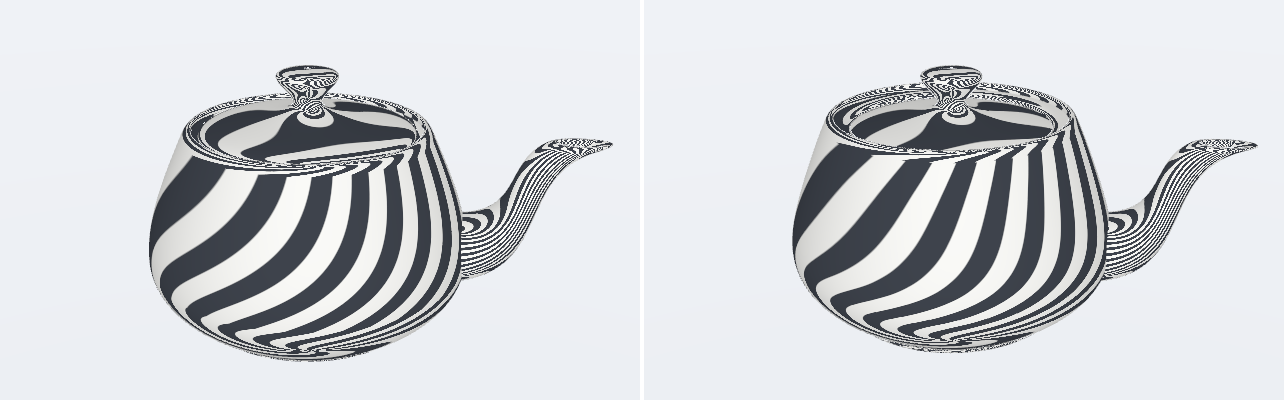
\includegraphics[width=\columnwidth]{figures/fig_reflection.png}
\caption{Reflection lines. Left: the 1976 lattice; the stripes bend where
the upper and lower body meet. Right: the 2026 lattice from samples.}
\label{fig:reflect}
\end{figure}

The picture is kinder than the numbers, and the numbers are the result.
At every joint between two exterior lattices we compared the two
surfaces' normals and the curvature of the curve that crosses the joint
(Table~\ref{tab:joints}). The sampled 2026 lattices keep the normal to
$0.11^\circ$ on average and $0.83^\circ$ at worst. They do not keep the
curvature: its relative jump across a joint averages 0.16, about what the
1976 patches have by design. The reason is the seam. Each lattice ends
with one-sided stencils, whose second derivative is accurate to second
order only, so two lattices that sample one $G^2$ surface still disagree
about its curvature at their common edge. Our 2026 teapot therefore has
the shape of Yuksel's, to the accuracy below, and approximately its
normals, but it is not itself curvature continuous. Lattices that run
across the smooth joints without a seam would be, where the limiter is
inactive; they need samples whose spacing is compatible across the joint,
which the generator's meshes do not promise. We leave that open.

\begin{table}[H]
\caption{Across the joints of exterior lattices, 9 by 9 nodes each}
\label{tab:joints}
\centering
\scriptsize
\begin{tabular}{l|cc|cc}
\hline
 & \multicolumn{2}{c|}{Normal turn (deg)} & \multicolumn{2}{c}{Curvature jump}\\
Lattices & mean & max & max & mean rel.\\
\hline
1976, 44 joints & 0.06 & 1.71 & 2.85 & 0.19\\
2026, 52 joints & 0.11 & 0.83 & 49.4 & 0.16\\
\hline
\end{tabular}
\end{table}

The maximum for 1976 is the kink at the knob tip, and the large maximum
for 2026 is on the narrow tubes, where curvature itself is large.
\emph{Accuracy of the sampled shape.} We have no finer truth for the 2026
surfaces than the samples, so we hold some out: lattices built from every
other sample, $5\times5$ per patch, predict the omitted samples to
$2.1\times10^{-3}$ at worst and $6.6\times10^{-4}$ rms on the exterior
($3.7\times10^{-3}$ and $8.0\times10^{-4}$ on the interior), on a body
4.0 wide. The $9\times9$ lattices have half that spacing and
fourth-order ends, so their error should be near a sixteenth of these
figures; that is an expectation, not a measurement.

For the 1976 data alone the picture is as follows. Around the body
and lid, the round style has no seams, and one-sided finite differences
find no curvature jump across node lines (relative jump below
$2\times10^{-8}$). Along the profile, the exact and round styles copy the
original and therefore its curvature jumps: the worst is 2.85 in absolute
curvature, at the joint of the rim and the upper body. They are not
curvature continuous there, and Yuksel's construction \cite{yuksel2026}
is.

One might hope to obtain continuity by removing the seams along the
profile and leaving them only at true creases. We built that variant,
with rows graded in arc length so that spacing changes gradually. It is
not a success at the node counts of interest. At four intervals per patch
it deviates from the original by up to $4.0\times10^{-2}$, and it is not
smooth either: where the tight curl of the rim falls between nodes,
admission acts and leaves tangent turns of up to $13^\circ$ at node
rows, and the cap crease is rounded to $47^\circ$ where it should be
$90^\circ$. Doubling the nodes brings the deviation to about
$2\times10^{-2}$. A CONV lattice is smooth where its data are resolved
and it is honest about where they are not; it does not manufacture
curvature continuity at a feature it cannot see. The seamed styles are
the ones we recommend.

\subsection{What is not addressed}

The handle and spout still pass through the body in every version here; a
lattice has no notion of trimming, and the trimmed and chamfered surfaces
of the 1992 to 2026 models are not grids of samples. From outside the
difference is confined to the joins, where the 2026 chamfers make the
normal continuous and ours do not. In the 1975 to 1987 versions the lid
still floats 0.1 above the rim.

\subsection{No mesh}

Several options of the official page concern tessellation: duplicate
vertices along patch edges, triangles at the tips, matching normals
across edges, the direction of triangulation. A node lattice has one node
where patches meet, and Section~\ref{sec:transport} renders the surface
itself. At a pole the solver's damped step and a normal taken a short
distance along $v$ are the whole treatment.

\section{Rays by Transport}
\label{sec:transport}

A camera ray meets $S(u,v)$ where two scalar equations vanish. The usual
method searches for that point from the ray's side
\cite{kajiya1982,toth1985}: a hierarchy of bounds, then Newton's method.
\emph{Correspondence transport}, introduced for a cloth experiment built
on CONV, works from the surface's side. The parameters of a lattice of
surface points are known; where those points land on the screen tells
nearby pixels where their rays must meet the surface.

\subsection{Method}

\begin{enumerate}
\item \emph{Transport.} Evaluate each part on a lattice of $k$ samples per
node interval ($k=4$) and project the points.
\item \emph{Predict.} Each projected lattice cell, split into two
triangles and dilated by 0.6 pixel, gives every pixel centre it covers a
candidate $(u,v)$ by barycentric interpolation, with a lower bound on
depth. A pixel keeps up to six candidates in depth order. Workers own
disjoint bands of rows, so the lists need no locks and their order is
deterministic.
\item \emph{Correct.} In depth order, a pixel refines a candidate on the
true surface by Newton's method with the dual-number derivatives, to
0.01 pixel. It stops at the first converged hit that is nearer than the
next candidate's bound.
\end{enumerate}
No ray searches anything. The triangles are predictors only; every hit,
normal and texture coordinate comes from the surface.

Two refinements carry most of the gain. A prediction whose first residual
is under 0.35 pixel takes one exact Newton step and is accepted without a
second evaluation, provided the step stays inside one cell and is not
long for its residual, which excludes creases and grazing rays; the
error of such a step is of second order in the residual. And a solve that
fails to halve its residual after two iterations is abandoned; without
this, rays that just miss a silhouette cost eight evaluations each and
dominate the frame.

\subsection{Comparison}

The baseline traces each ray independently through a bounding-volume
hierarchy over the \emph{same} lattice cells, intersects the same two
triangles per cell, and corrects with the same solver and the same
one-step rule. It is a strong baseline: it differs from transport only in
how a ray finds its candidates. Table~\ref{tab:render} gives medians of
21 frames of the exact teapot on an Apple A18 Pro (six cores), Apple
clang 21 at \texttt{-O3} without contraction. The machine was shared
during the measurements (load average near 6), so the absolute times are
indicative and the ratios are the result.

\begin{table}[H]
\caption{Frame time (ms), one sample per pixel}
\label{tab:render}
\centering
\scriptsize
\begin{tabular}{ll|rr|c}
\hline
Frame & Threads & Transport & Per ray & Ratio\\
\hline
$640\times400$ & all & 17.4 & 29.1 & 1.67\\
$640\times400$ & one & 48.4 & 87.4 & 1.81\\
$960\times600$ & all & 30.3 & 59.6 & 1.97\\
$960\times600$ & one & 90.9 & 221.4 & 2.44\\
\hline
\end{tabular}
\end{table}

The mechanism is visible in the counters. At $960\times600$ transport
starts 1.09 solves and makes 1.34 surface evaluations per surface pixel;
the per-ray tracer starts 1.90 and makes 2.10, and visits 8.5 hierarchy
nodes per ray besides. Transport pays 4.8\,ms to predict and 4.7\,ms to
transport the lattice and build the shadow map. A repeat of the last row
gave 183\,ms for the per-ray tracer, so that ratio should be read as
about two.

\emph{Agreement.} For the $960\times600$ frame we re-evaluated every
reported $(u,v)$: the worst reprojection error is 0.20 pixel and the mean
$5\times10^{-4}$ pixel. Against a per-ray reference with a lattice four
times finer and no one-step rule, transport agrees on 98{,}347 of 98{,}462
surface pixels (99.88\%) and the per-ray tracer on 98{,}349. Nearly all
the differences lie on silhouettes and crease edges, where a ray grazes
two roots less than a pixel apart and neither method is certain to return
the nearer. Neither proves that every intersection has been found.

\subsection{Edges, floor, and gloss}

\emph{Edges.} One sample per pixel leaves stair-stepped silhouettes. A
pixel whose neighbour shows another part, another sheet or no surface
receives four more samples on a rotated grid, which reuse the pixel's
own predictions. About 2\% of pixels qualify, but their rays are the
expensive ones, and the frame costs about twice as much: 40.0\,ms against
50.4\,ms per ray at $640\times400$ on all threads.

\emph{Floor.} The view reflected in a planar floor is the view from the
eye mirrored in that plane, an identity used for planar mirrors in an
earlier photonic transport experiment. Its rays are as coherent as the
camera's, so the reflection is one more transport pass from the mirrored
eye over the same lattice.

\emph{More surfaces.} The 2026 version has 66 lattices and 5346 nodes,
with interior sheets behind most exterior pixels. A $640\times400$ frame
of it takes 38.6\,ms by transport and 55.8\,ms per ray without edge
samples, and 61.1\,ms and 80.3\,ms with them.

\emph{Gloss.} A ray reflected by the curved teapot is not coherent with
its neighbours, and transport has nothing to offer it; those rays go
through the per-ray tracer, one bounce. The emitter is a rectangle seen
along the reflected ray, so a highlight has the shape of a window and not
of a point light's lobe. With gloss and a polished floor a $640\times400$
frame takes 72.9\,ms by transport and 96.7\,ms per ray, edge samples
included.

\emph{Wireframe and texture.} A hit carries its own $(u,v)$ and their
screen gradients, so node lines and patch outlines are drawn in the
shader with hidden lines removed for free, and they are curves on the
surface, not a cage around it. Textures are small RGB lattices
reconstructed by the same CONV evaluator, mapped per part or per patch as
on the 1976 journal cover \cite{blinnnewell1976}.

Fig.~\ref{fig:looks} shows four renderings and Fig.~\ref{fig:work} the
solver work per pixel.

\begin{figure*}[t]
\centering
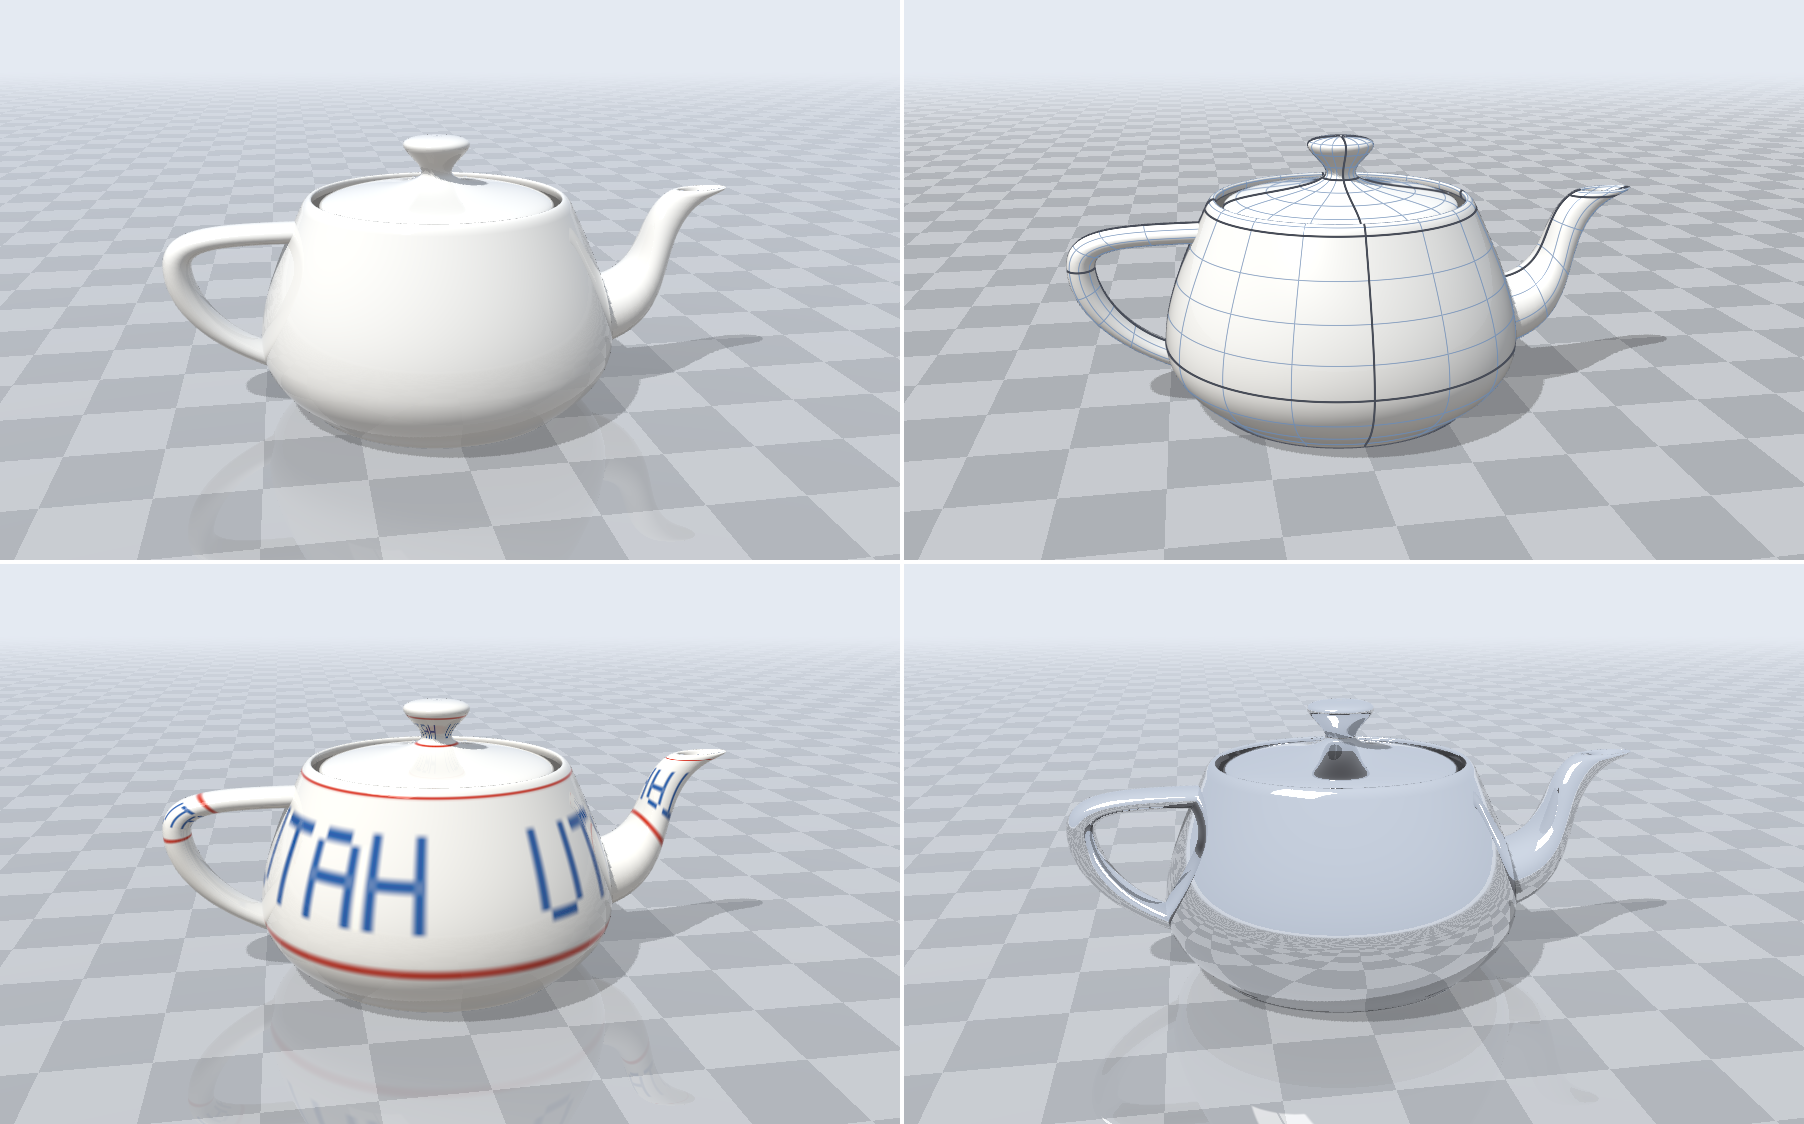
\includegraphics[width=0.92\textwidth]{figures/fig_looks.png}
\caption{The CONV teapot, exact style, 560 nodes, traced by transport.
Top: porcelain with gloss on a polished floor; node lines (thin) and the
original patch outlines (heavy) drawn from the hit parameters. Bottom: a
low-resolution texture magnified by CONV under a traced glaze; chrome,
reflecting the floor and its own handle and spout.}
\label{fig:looks}
\end{figure*}

\begin{figure}[t]
\centering
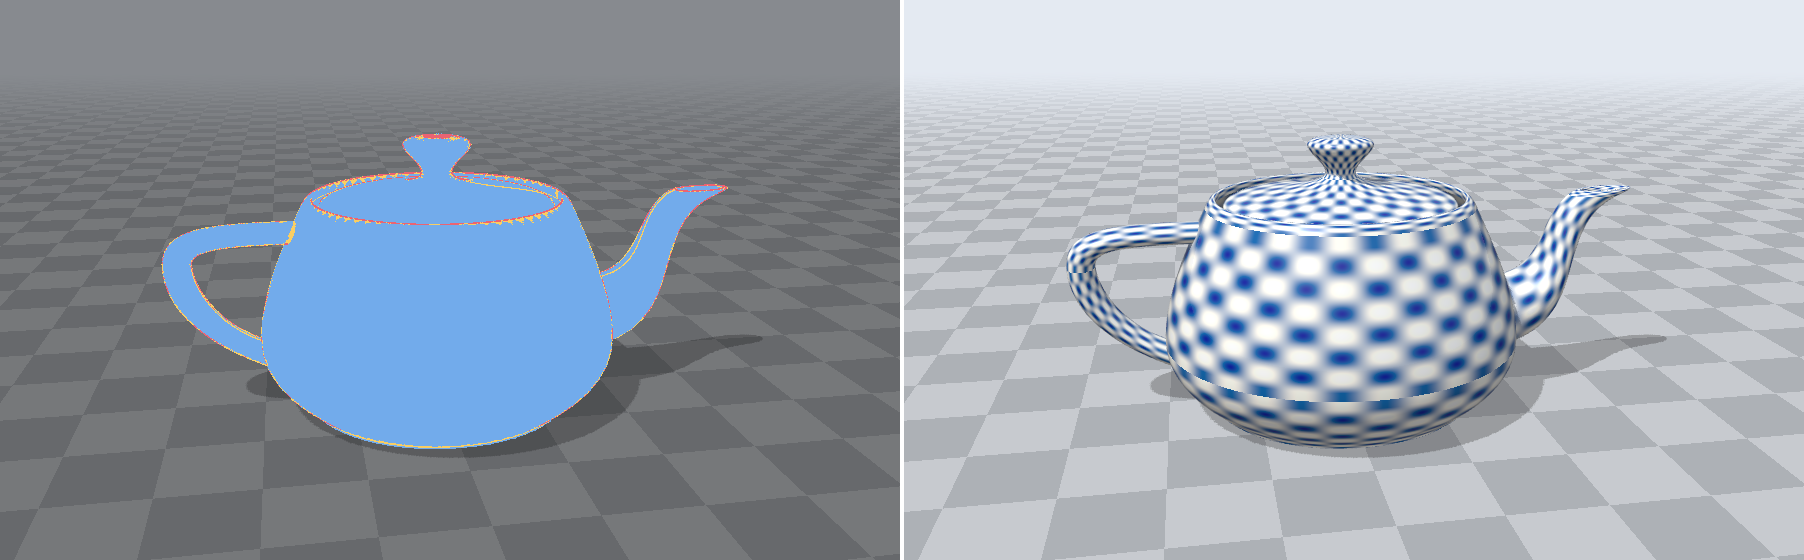
\includegraphics[width=\columnwidth]{figures/fig_work.png}
\caption{Left: solver work. Blue pixels needed one solve, orange two, red
more. Right: a checker mapped in patch coordinates.}
\label{fig:work}
\end{figure}

\section{Motion}

Since every node is a surface point, the collision shape of the teapot
can be taken from the lattice with no separate model: the convex hull of
a group of nodes is a convex piece of the teapot. For the 1975 to 1987
versions we use eleven hulls, one for the body, two for the lid, and four
each along the handle and spout; for the 2026 version, one hull per
group of exterior lattices. We hand them to the rigid-body engine of a rock-stacking game,
whose wrench-transport solver resolves contact, friction and rolling
resistance in one solve per frame. One model unit is taken as 7\,cm. The
engine returns a pose; the pose is applied to the rest nodes and the
surface is recompiled through them, which takes 0.17\,ms. Dropped from 42\,cm at a tilt of 1.2\,rad, the teapot lands on its
spout, rocks back over its base and is asleep within 1.5\,s
(Fig.~\ref{fig:drop}). The body is treated as solid porcelain, which is
not how a teapot is made; a shell would need the interior that this model
lacks.

\begin{figure*}[t]
\centering
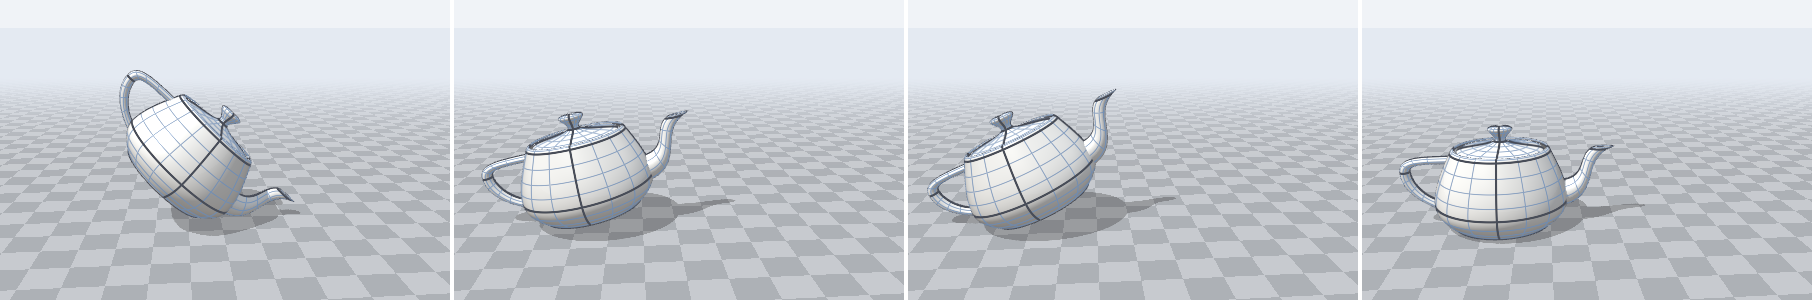
\includegraphics[width=0.92\textwidth]{figures/fig_drop.png}
\caption{A drop, at 0.30, 0.42, 0.60 and 1.60\,s. The surface is
rebuilt through the moved nodes at every frame.}
\label{fig:drop}
\end{figure*}

\section{Limits}

The variation bound is factorwise and coordinatewise; it does not bound
the curvature of the surface or forbid self-intersection. Exact
reproduction is a statement about a rest pose whose admission is
inactive; a deformed lattice is a CONV surface through the moved nodes,
not a deformed B\'ezier surface. The surface is continuous within a part
and only there. Transport and the per-ray tracer both accept a converged
root without proving it the nearest, and both use lattice triangles as
predictors, so a feature thinner than a lattice cell on screen can be
missed. The hierarchy's boxes are padded by a fraction of their diagonal,
which is a heuristic and not an enclosure. Timings are of one
implementation on one shared machine. In a browser the engine runs on one
thread in WebAssembly at about 80\,ms for a plain $640\times400$ frame
without edge samples.

\section{Conclusion}

Put on a CONV lattice with seams, the Utah Teapot is the same surface it
was in 1976, held by 560 points that lie on it. The lattice can be made
round by moving nodes onto circles, traced without a mesh, textured in
its own parameters, and dropped on a floor by handing its nodes to a
physics engine. Later versions enter as samples, with no knowledge of how
they were constructed: the 2026 teapot, interior included, is 66 small
lattices. What the lattices do not carry across their seams is curvature
continuity, and they do not carry trimming or chamfers at all. Those are
the places where the later teapots, and Yuksel's in particular, did work
that this representation does not replace. A seamless lattice over
compatibly spaced samples of a $G^2$ surface is the experiment we would
do next.

\section*{Attribution}

The Utah Teapot was created by Martin Newell at the University of Utah
and scaled by Jim Blinn; the 1987 bottom is Frank Crow's and the 2026
version is Cem Yuksel's. The models built here are Modified Utah Teapots
in the sense of the terms on the official page \cite{utahpage}: the 1976
surface re-expressed, with an optional flat cap; and surfaces of the 1987
and 2026 versions rebuilt from points sampled with that page's mesh
generator, without trimming or chamfers.

\section*{AI Generated Work Disclaimer}

Substantial portions of this work were generated with the assistance of
Anthropic Claude models.

\begin{thebibliography}{9}
\scriptsize
\bibitem{newell1975}
M. E. Newell, ``The utilization of procedure models in digital image
synthesis,'' Ph.D. dissertation, Univ. of Utah, Salt Lake City, UT, USA,
1975.
\bibitem{blinnnewell1976}
J. F. Blinn and M. E. Newell, ``Texture and reflection in computer
generated images,'' \emph{Commun. ACM}, vol. 19, no. 10, pp. 542--547,
Oct. 1976.
\bibitem{crow1987}
F. Crow, ``The origins of the teapot,'' \emph{IEEE Comput. Graph. Appl.},
vol. 7, no. 1, Jan. 1987.
\bibitem{blinn1987}
J. F. Blinn, ``What, teapots again?'' \emph{IEEE Comput. Graph. Appl.},
vol. 7, no. 9, Sep. 1987.
\bibitem{utahpage}
``The Utah Teapot,'' Univ. of Utah.
\url{https://graphics.cs.utah.edu/teapot/} (accessed Nov. 11, 2026).
\bibitem{yuksel2026}
C. Yuksel, ``Continuity-enhancing degree elevation and splits,'' in
\emph{Proc. SIGGRAPH}, 2026, as cited on \cite{utahpage}.
\bibitem{utahdata}
``Utah Model Repository: Original Bezier Teapot,'' Univ. of Utah.
\url{https://users.cs.utah.edu/~dejohnso/models/teapot.html} (accessed
Nov. 11, 2026).
\bibitem{convpaper}
``Compact Ordered Nodal Variation,'' 2026.
\url{https://github.com/malkuth-software/papers}.
\bibitem{kajiya1982}
J. T. Kajiya, ``Ray tracing parametric patches,'' in \emph{Proc.
SIGGRAPH}, 1982, pp. 245--254.
\bibitem{toth1985}
D. L. Toth, ``On ray tracing parametric surfaces,'' in \emph{Proc.
SIGGRAPH}, 1985, pp. 171--179.
\end{thebibliography}
\end{document}
